% %
% main.tex
%

% notes = hide | show | only
\documentclass[xcolor=dvipsnames,dvip,notes=show,table]{beamer}

% Para crear una versión 'handout' (impresa)
%\documentclass[xcolor=pst,dvips,handout,notes=show]{beamer}

%
% cabeceras.tex
%

\usepackage[T1]{fontenc}

 \definecolor{ZurichBlue}{rgb}{.255,.41,.884}
 \beamertemplateshadingbackground{white!10}{white!10}
%\usepackage{beamerthemeWarsaw}

% \usepackage{longtable}
\usepackage{beamerthemeBoadilla}


%\usepackage{tikz,times}
\usetheme{boxes}
%\usepackage{handoutWithNotes}
\usepackage{pgfpages}
%\pgfpagesuselayout{2 on 1}[a4paper,border shrink=5mm]


%\usecolortheme[named=OliveGreen]{structure} 
\setbeamertemplate{items}[ball] 
%\setbeamertemplate{blocks}[rounded][shadow=true] 
\setbeamertemplate{footline}[page number]
\addtocounter{framenumber}{-1}
%Handout



%\usepackage{beamertheme}
%\usepackage{beamerthemeshadow}
\useoutertheme[hooks]{tree}
 
% \setbeamertemplate{headline}[default] % The default is just an empty headline.
% \setbeamertemplate{headline}[infolines theme]
% \setbeamertemplate{headline}[miniframes theme]
% \setbeamertemplate{headline}[sidebar theme]
% \setbeamertemplate{headline}[smoothtree theme]
% \setbeamertemplate{headline}[smoothbars theme]
% \setbeamertemplate{headline}[tree]
\beamertemplatetransparentcovereddynamic
% spanish
\usepackage[spanish]{babel}
\usepackage[utf8]{inputenc}

% diagramas
%\usepackage{pst-eps,epstopdf}
\usepackage{pst-node}
%\usepackage{pst-all}
\usepackage{pst-blur}
%\usepackage{pst-tree}

% incrustaciones de código fuente
\usepackage{listings}

% matemáticas y símbolos
\usepackage{amsmath}
\usepackage{amssymb}
\usepackage[right]{eurosym}
\usepackage{ulem}

% colores
\usepackage{colortbl}

%\usepackage{algorithm2e}
%\usepackage{algorithm}
%\usepackage{algorithmic}

\lstset{language=[90]Fortran,
  basicstyle=\ttfamily,
  keywordstyle=\color{darkred},
  commentstyle=\color{green},
  frame=trBL,
  stringstyle=\color{violet},
  frameround=tttt,
  backgroundcolor=\color{lightyellow},
  morecomment=[l]{!\ }% Comment only with space after !
}


% 
% \lstset{%
%   language=Fortran,
% 	basicstyle=\footnotesize\sffamily,
% 	keywordstyle=\color{darkred}
%  	stringstyle=\color{violet}
%  	commentstyle=\color{blue}
%  	showspaces=false,
%  	showtabs=false,
%  	showstringspaces=false,
%  	frame=trBL,
%         frameround=tttt,
%         backgroundcolor=\color{lightyellow},
%  	extendedchars=true,
%  	numbers=none,
%         aboveskip=0.5cm,
%         belowskip=0.5cm,
%         xleftmargin=1cm,
%         xrightmargin=1cm,
% 	breaklines=true
% }
\definecolor{darkred}{rgb}{0.5, 0, 0}
\definecolor{violet}{rgb}{1, 0, 1}
\definecolor{lightyellow}{rgb}{1,1,0.8}


\usepackage{latexsym}
\usepackage{amsmath}
\usepackage{amssymb}
\usepackage{amsthm}

\usepackage{xspace}



\hyphenation{real}

\newrgbcolor{ColorEncabezadoTabla}{0.7 0.7 0.9}
\newrgbcolor{ColorFila1}{0.8 0.8 0.7}
\newrgbcolor{ColorFila2}{0.8 0.7 0.8}
\newrgbcolor{ColorTotal}{0.7 0.9 0.7}


% \usepackage{tikz,times}
% \usetikzlibrary{mindmap,backgrounds}



%%%%%%%%%%%%%%%%%%%%%%%%%%%%%%%%%%%%%%%%%%%%%%%%%%%%%%%%%%%%%%%%%%%%%%

\title[The CORFU technique | MTSR 2013]{Towards a stepwise method for unifying and reconciling corporate names in public contracts metadata. \\ The CORFU technique.}
\author[Jose María Álvarez Rodríguez]{\textbf{Michalis Vafopoulos} (speaker) \\ and \\ \{Jose María Álvarez-Rodríguez, Patricia Ordoñez De Pablos and \\ Jose Emilio Labra-Gayo\}}
\institute{MTSR 2013 | 7th Metadata and Semantics Research Conference \\ Track on Metadata and Semantics for Open Repositories, Research Information Systems and Data Infrastructures}


\date{}

\begin{document}

\frame{
\titlepage

}

\frame{
\tableofcontents

}


\section{Introduction}

\frame{
  \frametitle{The Problem...} 
}


\frame{
  \frametitle{Motivation and Rationale} 
}

\frame{
  \frametitle{Main Contributions} 
}


\section{Related Work}

\frame{
  \frametitle{Metadata in Public Contracts} 
}


\frame{
  \frametitle{Reconciling names} 
}

\section{The CORFU technique}

\frame{
  \frametitle{Overview} 
}

\frame{
  \frametitle{Example} 
}

\frame{
  \frametitle{Step 1: FIXME} 
}


\section{Use Case: the PublicSpending initiative}

\frame{
  \frametitle{Overview} 
}

\frame{
  \frametitle{The CORFU technique in Action...} 
}


\section{Evaluation and Discussion}

\frame{
  \frametitle{Design of the experiment} 
}



\frame{
  \frametitle{Results} 
}


\frame{
  \frametitle{Graphical view of initial results without applying the CORFU technique...}
\begin{figure}[htb]
\centering
	
\includegraphics[width=6cm]{imgs/previous-corfu}
%\caption{Modelo $5\star$ (W3C).}
\end{figure}

  }
  

  \frame{
  \frametitle{Graphical view after applying the CORFU technique...}
\begin{figure}[htb]
\centering
	
\includegraphics[width=6cm]{imgs/corfu-stats}
%\caption{Modelo $5\star$ (W3C).}
\end{figure}

  }
  
  
  
  \frame{
  \frametitle{Graphical view after applying the CORFU technique to the first 100 Forbes companies...}
\begin{figure}[htb]
\centering
	
\includegraphics[width=6cm]{imgs/corfu-forbes-100}
%\caption{Modelo $5\star$ (W3C).}
\end{figure}

  }
  
  
    \frame{
  \frametitle{...the first 100 Forbes companies in bubbles...}
\begin{figure}[htb]
\centering
	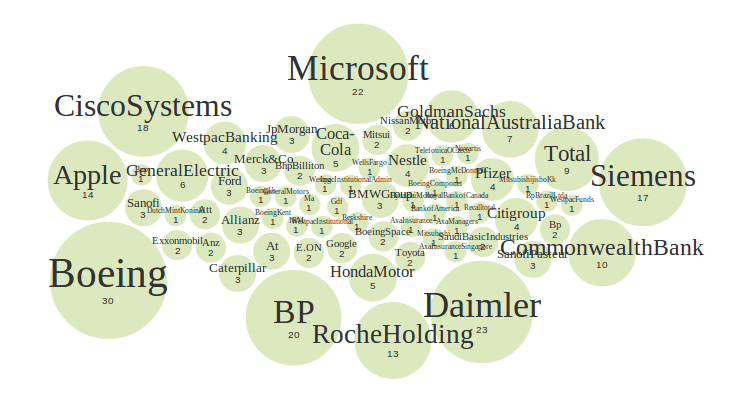
\includegraphics[width=10cm]{imgs/forbes}
%\caption{Modelo $5\star$ (W3C).}
\end{figure}

  }
  
  
  
\frame{
  \frametitle{Advantages} 
}


\frame{
  \frametitle{Restrictions} 
}



\section{Conclusions and Future Work}

\frame{
  \frametitle{Conclusions} 
}


\frame{
  \frametitle{Future Work} 
}




\section*{End of the presentation...}

\frame{
    
  \begin{figure}[!htb]
\centering
 
\includegraphics[width=9cm]{imgs/thanks}
\end{figure}


}



\section{Metadata and Information}


\frame{
  \frametitle{Roster...} 
  
  \begin{table}[!htb]

\scriptsize
\begin{center}
\begin{tabular}{p{3cm} p{7cm}}
  \begin{figure}[!htb]
\centering
 
\includegraphics[width=1cm]{imgs/chema}
\end{figure} & \begin{itemize}
                \item Dr. Jose María Alvarez-Rodríguez
                \item SEERC (until August, 2013) and Carlos III University of Madrid, Spain
                \item E-mail: \url{josemaria.alvarez@uc3m.es}
                \item WWW: \url{http://www.josemalvarez.es}
               \end{itemize} \\

\begin{figure}[!htb]
\centering
 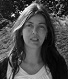
\includegraphics[width=1cm]{imgs/patriop}
\end{figure} & \begin{itemize}
                \item Prof. Dr. Patricia Ordoñez De Pablos
                \item University of Oviedo, Spain
                \item E-mail: \url{patriop@uniovi.es}
               \end{itemize} \\
               

\begin{figure}[!htb]
\centering
 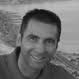
\includegraphics[width=1cm]{imgs/labra}
\end{figure} & \begin{itemize}
                \item Prof. Dr. Jose Emilio Labra-Gayo
                \item University of Oviedo, Spain
                \item E-mail: \url{labra@uniovi.es}
                \item WWW: \url{http://www.di.uniovi.es/~labra}
               \end{itemize}
               \end{tabular}
  \end{center}
\end{table} 

  
}



\appendix



\section*{References}
\bibliographystyle{abbrv}
\tiny
\bibliography{references}


% %%%%%%%%%%%%%%%%%%%%%%%%%%%%%%%%%%%%%%%%%%%%%%%%%%%%%%%%%%%%%%%%%%%%%%

\normalsize

\frame{
\titlepage

}

% %%%%%%%%%%%%%%%%%%%%%%%%%%%%%%%%%%%%%%%%%%%%%%%%%%%%%%%%%%%%%%%%%%%%%%

\end{document}
